\documentclass[addpoints]{exam}

\makeatletter % Lagfæring fyrir nýjar útgáfur af TeXLive
\expandafter\providecommand\expandafter*\csname ver@framed.sty\endcsname
{2003/07/21 v0.8a Simulated by exam}
\makeatother

\usepackage[top=2cm, bottom=2cm, left=1cm, right=1cm]{geometry}
\usepackage[utf8]{inputenc}
\usepackage[icelandic]{babel}
\usepackage[T1]{fontenc}
\usepackage[sc]{mathpazo}
%\usepackage{helvet} \renewcommand\familydefault{\sfdefault}
\usepackage[parfill]{parskip}
\usepackage{booktabs,tabularx}
\usepackage{multirow}
\usepackage{multicol}
\usepackage{vwcol}
\usepackage{graphicx}
\usepackage{amsmath, amsfonts, amssymb, amsthm}
\usepackage{minted} %Minted and configuration
\usepackage{afterpage}
\usepackage{scrextend}

\usepackage[pdftex,bookmarks=true,colorlinks=true,pdfauthor={Eirikur Ernir Thorsteinsson},linkcolor=blue,urlcolor=blue]{hyperref}

\setcounter{secnumdepth}{-1} 
\hyphenpenalty=5000

\newcommand\blankpage{%
    \null
    \thispagestyle{empty}%
    \addtocounter{page}{-1}%
    \newpage}

\usemintedstyle{default}
\renewcommand{\theFancyVerbLine}{\sffamily \arabic{FancyVerbLine}}
\author{}
\date{}

\footer{}{}{}

\setcounter{secnumdepth}{-1} 

\qformat{\large \textbf Question \thequestion \phantom{M}(\totalpoints \phantom{l}stig) \hfill}
\renewcommand{\solutiontitle}{\noindent\textbf{Svar:}\par\noindent}
\renewcommand{\points}{points}
\renewcommand{\questionshook}{\setlength{\itemsep}{0.5cm}}
%\hqword{Spurning:}
%\hpword{Stig í boði:}
%\hsword{Stig:}
%\htword{Samtals}

\title{TÖL105G Computer Science 1a - Final Exam}
\author{}
\date{18. december 2017}

\pagestyle{headandfoot}
\firstpageheader{TÖL105G -\\ Tölvunarfræði 1a}{Final Exam}{18. december 2017}
\firstpagefooter{}{Page. \thepage\ of \numpages}{}
\runningfooter{}{Page. \thepage\ of \numpages}{}
\setlength{\columnsep}{0.5cm}

\changefontsizes{14pt}

% \printanswers
\begin{document}

% \thispagestyle{empty}
Fullt nafn: \vspace*{1mm} \hrule
\vspace*{0.5cm}

\begin{center}
\begin{minipage}{.8\textwidth}
This exam contains \numquestions\ worth a total of \numpoints\ points.

Write your answers on these pages.

You may bring a calculator and one A4 sheet of notes to the exam.
\end{minipage}
\end{center}

\vspace{1cm}

\begin{questions}

\question Multiple choice questions. Carefully mark one option in each question. 

Points are not deducted for wrong answers.

\begin{parts}
\part[3] The statement
\begin{minted}{matlab}
>> x = '1' < 1;
\end{minted}
is entered into the Matlab Command Window. What is the type of the variable \texttt{x}?

\begin{oneparcheckboxes}
    \choice \texttt{int32}
    \choice \texttt{double}
    \CorrectChoice \texttt{logical}
    \choice \texttt{char}
    \choice Matlab throws an error.
\end{oneparcheckboxes}

\part[3] The statement

\begin{minted}{matlab}
>> y = 3 > 2 > 1   
\end{minted}
is entered into the Matlab Command Window. What is the value of \texttt{y}?

\begin{oneparcheckboxes}
    \CorrectChoice \texttt{0}
    \choice \texttt{1}
    \choice \texttt{[0 1]}
    \choice \texttt{[1 0]}
    \choice Matlab throws an error.
\end{oneparcheckboxes}

\part[3] How many times does the program segment to the side run?
\begin{multicols}{2}
\begin{checkboxes}
\choice Never
\choice Once
\CorrectChoice Four times
\choice Eight times
\choice An infinite number of times
\end{checkboxes}

\begin{minipage}{0.8\linewidth}
\begin{minted}[frame=lines]{matlab}
x = 1;
while x < 16
    disp('The loop ran!')
    x = x*2;
end
\end{minted}
\end{minipage}
\end{multicols}

\part[3] Which of the following is a floating point type in Matlab?

\begin{oneparcheckboxes}
    \choice \texttt{int32}
    \CorrectChoice \texttt{double}
    \choice \texttt{logical}
    \choice \texttt{char}
    \choice \texttt{float}
\end{oneparcheckboxes}

\vspace*{1.5cm}
\hspace{0.8cm}
\gradetable[h][questions]
\part[3] A cell array is given:
\begin{minted}{matlab}
c = {1, 2, {3, 4, [5, 6]}};
\end{minted}
Which of the following commands gives the value \texttt{5}?

\begin{checkboxes}
    \choice \verb|c(3){3}{1}|
    \choice \verb|c{3}(3){1}|
    \choice \verb|c(3)(3){1}|
    \choice \verb|c{3}(3)(1)|
    \CorrectChoice \verb|c{3}{3}(1)|
\end{checkboxes}

\part[3] Which of the following command creates the structure \texttt{persona} with the field \texttt{nafn} and the value \texttt{'Gunna'}?

\begin{checkboxes}
    \choice \verb|persona = persona.nafn('Gunna')|
    \CorrectChoice \verb|persona.nafn = 'Gunna'|
    \choice \verb|persona = struct('Gunna','nafn')|
    \choice \verb|struct(persona, 'Gunna', 'nafn')|
    \choice \verb|persona(nafn) = 'Gunna'|
\end{checkboxes}

\part[3] If the vectors $x$ and $y$ contain the coordinates of 10 points, what command gives the optimal 2nd degree polynomial approximating the points?
\begin{checkboxes}
\choice \texttt{polyval(x,y,2)}
\choice \texttt{polyfit(x,y,'parabola')}
\choice \texttt{interp2(x,y,2)}
\CorrectChoice \texttt{polyfit(x,y,2)}
\choice \texttt{interp1(x,y,2)}
\end{checkboxes}

\part[3] Which of the following statements gives the logical value \texttt{1} when the string \texttt{s} is \texttt{'abc'}?

\begin{checkboxes}
    \choice \texttt{s = 'abc'}
    \choice \texttt{s == 'abc'}
    \choice \texttt{s.equals('abc')}
    \choice \texttt{compare(s,'abc')}
    \CorrectChoice \texttt{strcmp(s,'abc')}
\end{checkboxes}

\part[3] What does \texttt{nargin} give when used inside a function?

\begin{checkboxes}
    \CorrectChoice The total number of input variables
    \choice A cell array of input variables
    \choice A cell array of output variables
    \choice The length of the cell array \texttt{varargin}
    \choice The same as \texttt{varargin}
\end{checkboxes}

\part[3] In Matlab it is possible to define a function in one statement as\ldots

\begin{checkboxes}
    \CorrectChoice an anonymous function
    \choice a recursive function 
    \choice a nested function 
    \choice a function function
    \choice a vector function
\end{checkboxes}

\end{parts}

\question Write Matlab-statements (one in each part) to perform the described operations. Each part gives one point instead of two points if correctly solved in more than one line.

\begin{parts}
\part[2] Create the $2 \times 4$ matrix \texttt{m} containing evenly distributed random floating point numbers in the range $]-3;3[$.
\vspace*{1.5cm}
\part[2] Create the variable $a$ which contains the mean of all elements of $m$.
\vspace*{1.5cm}
\part[2] Create the $2 \times 4$ logical matrix \texttt{lm} which contains the value ``true'' where the absolute value of the corresponding element of \texttt{m} is bigger than 2.
\vspace*{1.5cm}
\part[2] Turn \texttt{m} into a $4 \times 4$ matrix by appending a copy of the matrix to its bottom. (This would make rows 1 and 3 identical, as well as rows 2 and 4)
\vspace*{1.5cm}
\part[2] Remove the last column from \texttt{m}.
\vspace*{3cm}
\end{parts}

\begin{solution}
\begin{verbatim}
>> m = rand(2,4)*(3-(-3))-3;
>> a = sum(sum(m))/numel(m); % Eða bara mean(m);
>> lm = abs(m) > 2;
>> m = [m ; m];
>> m(:,end) = [];
\end{verbatim}
\end{solution}

\newpage

\question[10] 

\begin{multicols}{2}
Write a Matlab-program which asks the user to enter a number and writes the corresponding number of lines of the triangle to the right, which contains the positive integers in ascending order. The triangle should maintain its shape for no fewer than the first 99 numbers.
\begin{verbatim}
      >> trianglenumbers
      Enter a number: 6
       1 
       2  3 
       4  5  6 
       7  8  9 10 
      11 12 13 14 15 
      16 17 18 19 20 21
\end{verbatim}
\end{multicols}

\newpage

\question[10]

\begin{multicols}{2}
The file \texttt{heat.dat} is given, its format can be seen to the side. The first column represents a year, the second the average temperature in December that year.

Write Matlab-statements which read and plot the file contents. The years should be on the horizontal axis and the temperature on the vertical axis.

\begin{verbatim}
    
    
        2016 3.6
        2013 -0.5 
        2010 0.7
        2007 1.3
        ...  ...
    
    
\end{verbatim}
\end{multicols}

\begin{solution}
\begin{minted}[frame=lines] {matlab}
fid = fopen('arshiti.dat');
if fid ~= -1
    c = textscan(fid, '%f %f');
    ar = c{1};
    desemberhiti = c{2};
    plot(ar,desemberhiti);
end
fclose(fid);
\end{minted}
\end{solution}

\newpage

\question[10] Write the recursive function \texttt{recrev} which accepts a row vector and returns a vector where the order of its elements has been reversed.

Example:
\begin{verbatim}
>> recrev([1 2 3 4 5])
ans =
        5     4     3     2     1
\end{verbatim}

The function must be recursive. No more than half marks will be given to a solution which is not.

\paragraph{Note:} When a vector is of length 1 or less no work needs to be performed to reverse it. When it is of length 2 or more it can be reversed by switching the positions of the first and last elements and then applying the same function to the other elements.

\begin{solution}
\begin{minted}{matlab}
function r = recrev(v)
if length(v) <= 1
    r = v;
else
    r = [v(end) recrev(v(2:end-1)) v(1)];
end
end
\end{minted}    
\end{solution}

\newpage

\question[10]

\begin{multicols}{2}
Hazardous materials are marked using a black ``x'' on an orange background. Write Matlab-statements which draw this symbol.

The figure axes give an idea of coordinates to use when drawing.

The color orange can be created by combining 1 part red with 0.5 parts green and 0 parts of blue.

\begin{center}
    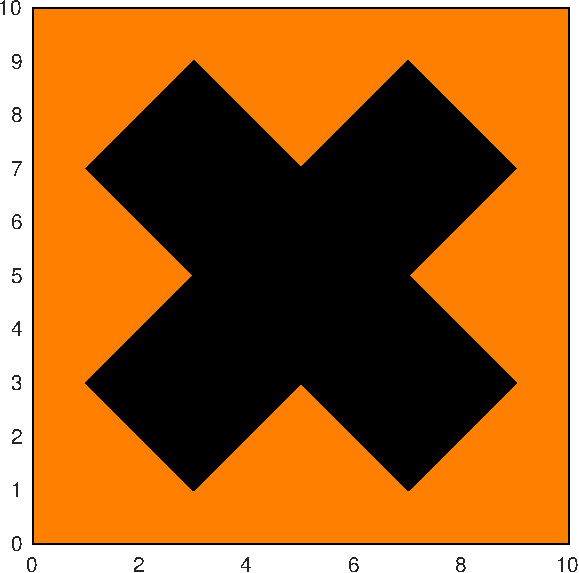
\includegraphics[width=0.8\linewidth]{Pics/haettulegtheilsu}
\end{center}

\end{multicols}

\newpage

\question[10] Write the Matlab class \texttt{Product} representing a product sold by weight. The class should have the properties \texttt{name} (e.g. ``clementines''), \texttt{priceperkg} and \texttt{unitsize} (e.g. 0.5 kg). Give the class a constructor and two additional methods - \texttt{unitprice} which returns the price of one unit and \texttt{increaseprice} which raises the price per kg by \texttt{p} percent.

\begin{solution}
    
\begin{minted}[frame=lines]{matlab}
classdef Product
    properties
        productname
        priceperkg
        unitsize
    end
    
    methods
        
        function p = Product(name, ppkg, unitsize)
            p.productname = name;
            p.priceperkg = ppkg;
            p.unitsize = unitsize;
        end
        
        function price = packageprice(p)
            price = p.priceperkg * p.unitsize;
        end
        
        function p = increaseprice(p, increase)
            p.priceperkg = p.pricepekg*(1+increase);
        end
        
    end
end
\end{minted}
   
\end{solution}

\newpage

\question[10] Definite integrals can be approximated by a method known as the trapezoidal rule. Divide the interval $[a,b]$ into $n$ evenly sized subintervals and calculate the area of a trapezoid for each subinterval. With a subinterval length of $h = (b-a)/n$ with boundaries at $x_i=a+ih$ with $i = 1,2,\ldots,n-1$ the rule is as follows:

\[
    \int_a^b f(x) dx \approx \frac{h}{2}\left(f(a) + 2f(x_1) + 2f(x_2) + \ldots + 2f(x_{n-1}) + f(b)\right)
\]

Write a function with accepts $f$ (as a function handle), $a, b$ and $n$ and calculates an integral according to the trapezoidal rule.

\end{questions}
\end{document}